\documentclass[11pt,a4paper,parskip=half]{scrartcl}
\usepackage{isabelle,isabellesym}

% further packages required for unusual symbols (see also
% isabellesym.sty), use only when needed

%\usepackage{amssymb}
  %for \<leadsto>, \<box>, \<diamond>, \<sqsupset>, \<mho>, \<Join>,
  %\<lhd>, \<lesssim>, \<greatersim>, \<lessapprox>, \<greaterapprox>,
  %\<triangleq>, \<yen>, \<lozenge>

%\usepackage[greek,english]{babel}
  %option greek for \<euro>
  %option english (default language) for \<guillemotleft>, \<guillemotright>

\usepackage[only,bigsqcap]{stmaryrd}
  %for \<Sqinter>

%\usepackage{eufrak}
  %for \<AA> ... \<ZZ>, \<aa> ... \<zz> (also included in amssymb)

%\usepackagetcomp}
  %for \<onequarter>, \<onehalf>, \<threequarters>, \<degree>, \<cent>,
  %\<currency>

% for uniform font size
%\renewcommand{\isastyle}{\isastyleminor}

% From src/HOL/HOLCF/document/root
\newcommand{\isasymnotsqsubseteq}{\isamath{\not\sqsubseteq}}

\usepackage{amsmath}
\usepackage{mathtools}
\usepackage{graphicx}
\usepackage{tikz}
\usepackage[T1]{fontenc}
\usepackage[utf8]{inputenc}
\usepackage{mathpartir}
\usepackage{calc}

% this should be the last package used
\usepackage{pdfsetup}

% urls in roman style, theorys in math-similar italics
\urlstyle{rm}
\isabellestyle{it}

% Isabelle does not like *} in a text {* ... *} block
% Concrete implemenation thanks to http://www.mrunix.de/forums/showpost.php?p=235085&postcount=5
\newenvironment{alignstar}{\csname align*\endcsname}{\csname endalign*\endcsname}
\newenvironment{alignatstar}{\csname alignat*\endcsname}{\csname endalignat*\endcsname}


\begin{document}

\title{The Correctness of Launchbury's Natural Semantics for Lazy Evaluation}
\author{Joachim Breitner\\
Programming Paradigms Group\\
Karlsruhe Institute for Technology\\
\url{breitner@kit.edu}}
\maketitle

\begin{abstract}
In his seminal paper „Natural Semantics for Lazy Evaluation“ \cite{launchbury},
John Launchbury proves his semantics correct with respect to a denotational
semantics. We have formalized both semantics and identified an ambiguity in
what the $\sqcup$ operator should do: If it is understood as the least upper
bound, as hinted at in the paper, the original proof fails.  We fix the proof
by taking a detour via a modified natural semantics with an explicit stack. In
addition, we show that the original proof goes through when $\sqcup$ is
understood to be a right-sided update.
\end{abstract}

\tableofcontents

\section{Introduction}

The Natural Semantics for Lazy Evaluation \cite{launchbury} created by John Launchbury in 1992 is often taken as the base for formal treatments of call-by-need evaluation, either to prove properties of lazy evaluation or as a base to describe extensions of the language or the implementation of the language. Therefore, assurance about the correctness and adequacy of the semantics is important in this field of research. Launchbury himself supports his semantics by defining a standard denotational semantics to prove both correctness and adequacy.

Although his proofs are already on the more rigorous side for pen-and-paper proofs, they have not yet been verified by transforming them to machine-checked proofs. The present work is a first step, formalizing both semantics in the proof assistant Isabelle and attempting to prove correctness. In the process we found a flaw in the original proof: Launchbury uses the operator $\sqcup$ in the natural semantics without giving a precise definition. If $\sqcup$ is understood to be the least upper bounds, then Theorem 2 in \cite{launchbury}, which is the generalization of the correctness statement used for Launchbury's inductive proof, is wrong. See Section \ref{sec_Correctness-Counterexample} for the counter example. Later publications based on Launchbury’s semantics reproduce the same flaw, often without the benefit of doubt that $\sqcup$ is supposed to be the least upper bound. Examples include \cite{nakata_extended}%
% (which is an extended version of \cite{nakata})
, \cite{distributed} and \cite{mixed}. 

To avoid the problem, we define an alternative natural semantics in Section \ref{sec_LaunchburyStacked} that carries more contextual information in the individual judgements. The added fields can be understood as the evaluation stack, carrying update frames and suspended application, hence the name “stacked semantics”.
This semantics is equivalent to the original one (\ref{sec_Launchbury-Unstack}) and provably correct (\ref{sec_CorrectnessStacked}).
While adding the stack does not affect the evaluation of expressions at all, e.g.\ is irrelevant for the semantics of the program, it does make the semantics more suited for formal proofs, as indicated by two observations:
\begin{itemize}
\item In the original semantics an explicit set of live variables has to be added to the judgements to be able to pick suitable fresh variables. This has been noted and fixed this way before, e.g.\ in \cite{sestoft}. In our new semantics, the additional fields contain all live variables and hence no special treatment is required.
\item To prove the correctness of the semantics inductively, the statement does not have to be generalized, but can be proved as-is.
\end{itemize}

Another approach to avoid the problem is to understand $\sqcup$, which operates on environments, to be a right-sided update:
\[
(\rho \sqcup \rho')(x) = 
\begin{cases}
\rho'(x), &\text{if } x \in \operatorname{dom} \rho' \\
\rho(x), &\text{otherwise.}
\end{cases}
\]
With this definition, the original proof goes through as written in \cite{launchbury}. We doubt that this reading is obvious or even intended, especially as the statement $\forall x. \rho(x) \sqsubseteq (\{\!\!\{\Gamma\}\!\!\})(x)$, given in \cite{launchbury} before the proof, is only true when $\sqcup$ is understood to be the least upper bound. The update-based definition has been used in other works that derive from Launchbury, e.g.\ in \cite{parallel} and \cite{nakata_blackhole}, but without further explanation of this choice.

Our contributions are:
\begin{itemize}
\item We define the natural and denotational semantics given by Launchbury in the theorem prover Isabelle.
\item In doing so we are, to our knowledge, the first to use both the Nominal package (to handle name binding) \cite{nominal} and the HOLCF \cite{holcf} package (for the domain-theoretic aspects) in the same development.
\item We identify a problem in the original correctness proof, and find two ways to fix it:
\begin{enumerate}
\item We define an alternative natural semantics with an explicit evaluation stack that simplifies the induction in the correctness proof and avoids the problem.
\item We show that the original proof goes through with a slight modification to the definition of the $\sqcup$-operator in the denotational semantics.
\end{enumerate}
\end{itemize}

%\subsubsection{The big picture}

The following picture gives an overview of the different semantics. Elements printed in black are formally defined and proved in the present work, while the gray square on the left shows the proofs and propositions in Launchbury’s original work \cite{launchbury}.

\begin{center}
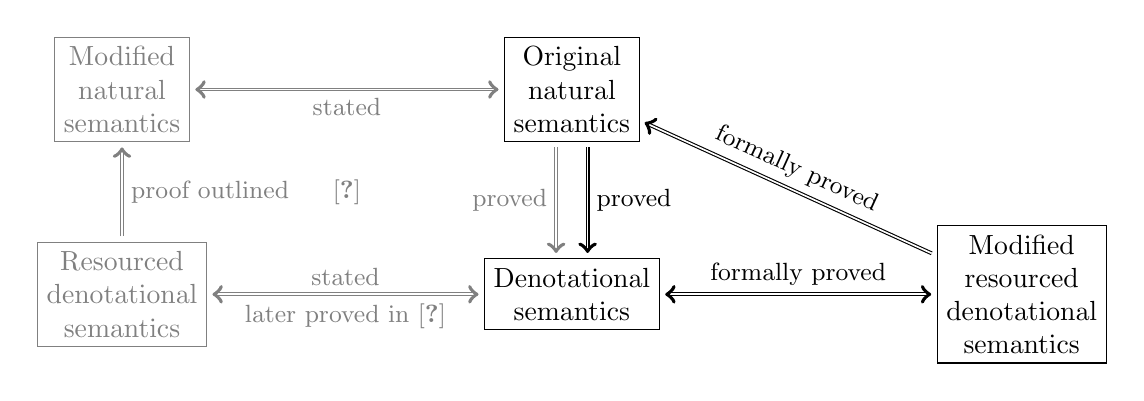
\begin{tikzpicture}[every node/.style={align=center}]
\matrix (m) [row sep=3em, column sep=10em] 
{ \node[draw,gray] (mn) {Modified\\natural\\semantics}; & \node[draw] (on) {Original\\natural\\semantics}; &; \\
  \node[draw,gray] (rd) {Resourced\\denotational\\semantics}; & \node[draw] (jd) {Denotational\\semantics}; & \node[draw] (sn) {Modified\\resourced\\denotational\\semantics} ;
  %\node[draw] (ud) {Denotational\\semantics\\with update};
  \\
};

\small
\draw[gray,<->,double, shorten <=.5ex, shorten >= .5ex]  (on) -- (mn) node[midway,below] {stated};
\draw[gray,->,double, shorten <=.5ex, shorten >= .5ex]  (rd) -- (mn) node[midway,right] {proof outlined};
\draw[gray,<->,double, shorten <=.5ex, shorten >= .5ex]  (rd) -- (jd) node[midway,above] {stated} 
                                                            node[midway,below] {later proved in \cite{functionspaces}};
\draw[transform canvas={xshift=2mm},->,double, shorten <=.5ex, shorten >= .5ex] (on) -- (jd) node[midway,right] {proved};
\draw[transform canvas={xshift=-2mm},gray,->,double, shorten <=.5ex, shorten >= .5ex] (on) -- (jd) node[midway,left] {proved};
\draw[<-,double, shorten <=.5ex, shorten >= .5ex]  (on) -- (sn) node[sloped,midway,above] {formally proved};
\draw[<->,double, shorten <=.5ex, shorten >= .5ex] (sn) -- (jd.east) node[sloped,midway,above] {formally proved};
%\draw[->,double, shorten <=.5ex, shorten >= .5ex] (on) -- (ud) node[sloped,midway,above] {Proof};
%\draw[<->,double, shorten <=.5ex, shorten >= .5ex]  (jd) -- (ud) node[midway,below] {formally proved};
\node[gray] at (barycentric cs:on=1,mn=1,rd=1,jd=1) {\cite{launchbury}};
\end{tikzpicture}
\end{center}


\input{Everything.tex}

\subsection{Related work}

Lidia Sánchez-Gil, Mercedes Hidalgo-Herrero and Yolanda Ortega-Mallén have worked on formal aspects of Launchbury’s semantics as well. On the one hand, they identified a step in his adequacy proof relating the standard and the resourced denotational semantics that is not as trivial as it seems at first and worked out a detailed pen-and-paper proof \cite{functionspaces}. They also plan to prove the equivalency between Launchbury’s natural semantics and a variant thereof, which was used by Launchbury in his adequacy proof, in the theorem prover Coq. As one step in that direction, they address the naming issues and suggest a mixed representation, using de Bruijn indices for locally bound variables and names for free variables \cite{nameless}. This corresponds to our treatment of names, using the Nominal logic machinery locally but not for names bound in heaps.

The same group extended Launchbury’s semantic for distributed lazy evaluation \cite{distributed}. In their modified natural semantics the heap retains the expression under evaluation with a special flag, marking them as blocked. Furthermore, the expression under evaluation has a name. Therefore the non-distributed subset of their semantics is very similar to our stacked semantics. This supports our claim that the stacked semantics is well suited for further proofs and extensions.

\begin{figure}
\begin{center}
\IfFileExists{session_graph.pdf}{
  \includegraphics[width=\textwidth]{session_graph}
}{Here, \texttt{session\_graph.pdf} would be shown.}
\end{center}
\caption{Theory Dependency Graph\label{theory-deps}}
\end{figure}

\subsection{Theory overview}

The following chapters contain the complete Isabelle theories, with one section per theory. Their interdependencies are visualized in Figure \ref{theory-deps}.

Chapter \ref{ch_aux} contains auxiliary theories, not necessarily tied to Launchbury's semantics. The base theories are kept independent of Nominal and HOLCF where possible, the lemmas combining them are in theories of their own, creatively named by appending \isa{-Nominal}, \isa{-HOLCF} or both.  You will find these theories:
\begin{itemize}
\item General utility functions extending Nominal (\isa{Nominal-Utils}).
\item A theory combining notions from HOLCF and Nominal, e.g.\ continuity of permutation (\isa{Nominal-HOLCF}).
\item A predicate for distinctly named associative lists (\isa{DistinctVars}, \isa{DistinctVars-Nominal}). 
\item A generalization of some parts of HOLCF to work on a set as a carrier instead of a type (\isa{HOLCF-Set}, \isa{HOLCF-Set-Nominal}).
\item Binary joins in the context of HOLCF (\isa{HOLCF-Join}).
\item A theory of fixed points of binary joins (\isa{HOLCF-Fix-Join}, \isa{HOLCF-Fix-Join-Nominal}).
\item A type for finite maps with a chain-complete partial order (\isa{FMap}, \isa{FMap-Nominal}, \isa{FMap-HOLCF}, \isa{FMap-Nominal-HOLCF}).
\item A function \isa{heapToEnv} that converts between associative lists and finite maps. (\isa{HeapToEnv})
\item The theory \isa{FMap-Utils} adds lemmas that combine finite maps with the various other non-standard auxiliary theories.
\end{itemize}

Chapter \ref{ch_natsem} defines Launchbury's natural semantics, while Chapter \ref{ch_natsemstack} provides the variant with the explicit stack and proves them equivalent.

Chapter \ref{ch_dendom} sets the stage for the denotational semantics by defining the denotational domain.

Chapter \ref{ch_denjoin} defines the denotational semantics where $\sqcup$ means the least upper bound. We show that Launchbury's Theorem 2 as stated is false for this semantics, and provide an alternative proof, that avoids the problematic generalization, via the stacked semantics. The semantics for heaps given in \isa{HSem} is abstract in the concrete type and denotation of expressions.

Chapter \ref{ch_denupd} defines the denotational semantics where $\sqcup$ means right-sided update, and proves Launchbury's semantics correct using the proof from his paper. The semantics can differ only for heaps; for expressions are assigned the same denotation. Again, the heap semantics in \isa{HSemUpd} is abstract in the concrete type and denotation of expressions.

\subsection{Reusable components}

Parts of this theory are independent of the actual semantics and may be of use to other users of Isabelle:

\subsubsection{Finite maps}

The theory \isa{FMap} defines maps with an explicit and finite domain. The need for this arises due to the combination of Nominal and HOLCF:

To effectively use the Nominal package, data types need to be in the \isa{fs} type class, indicating that they have finite support. Only then can the \isa{nominal-induct} method avoid the variables occurring in the support of a value when choosing bound names in the inductive step -- a crucial feature. Therefore, the usual data type for maps, \isa{var \isasymrightharpoonup{} value}, is insufficient. The obvious fix is to introduce a new type, \isa{var f\isasymrightharpoonup{} value} that contains only those maps with finite support.

But this causes issues with HOLCF: In order to work effectively with fixed points in HOLCF, the partial order for the type ought to have least upper bounds to all countable chains. With the usual order on partial maps, where binding additional variables makes the map larger, this is not possible in our type: Clearly the limit of a chain where at each step a new variable is added cannot have finite support.

Hence the partial order is changed so that only maps with the same domain are comparable. Assuming the values form a pointed chain-complete partial order (as it is the case here), we now have a chain-complete partial order on finite maps. Unfortunately, we now no longer have a bottom element for the whole type. In fact, the type is now the disjoint union of many pointed chain-complete partial orders, one for each domain. This makes proofs with fixed points relatively unwieldy, as we have to handle the domains of the maps explicitly. The theory \isa{HOLCF-Set} defines the notion of a set forming a pcpo and provides variants of some HOLCF functions to work with an explicit carrier set instead of the whole universe of the type. It also introduces the type class \isa{subpcpo-partition} for types that are disjoint unions of pcpos.

\subsubsection{Binary Joins in HOLCF}

The theory \isa{HOLCF-Join} defines the binary join operator $\sqcup$ in a partial order as defined by HOLCF, together with the \isa{compatible} predicate, expressing that the least upper bound exists for its arguments. It also contains type classes for the existence of meets (greatest lower bounds) in various settings and a proof that bifinite domains with meets for all finite nonempty sets have meets for arbitrary nonempty sets.

\subsection{Acknowledgement}

I’d like to thank Andreas Lochbihler for his gladly given and very effective help during the development of this theory. I’d also like to thank Brian Huffmann and Christian Urban for their help on HOLCF and Nominal, respectively. This work was supported by the Deutsche Telekom Stiftung.

\clearpage
\newcommand{\theory}[1]{\subsection{#1}\label{sec_#1}\input{#1.tex}}

\section{Auxillary theories}

\label{ch_aux}

\theory{Nominal-Utils}

% \theory{HOLCF-Utils}

\theory{Nominal-HOLCF}

\theory{DistinctVars}

\theory{DistinctVars-Nominal}

\theory{HOLCF-Set}

\theory{HOLCF-Join}

\theory{HOLCF-Set-Nominal}

\theory{HOLCF-Fix-Join}

\theory{HOLCF-Fix-Join-Nominal}

\theory{FMap}

\theory{FMap-Nominal}

\theory{FMap-HOLCF}

\theory{FMap-Nominal-HOLCF}

\theory{FMap-Utils}

\theory{HeapToEnv}

\clearpage
\section{Launchbury's natural semantics}
\label{ch_natsem}

\theory{Terms}
\theory{Heap}

\theory{Launchbury}

\clearpage
\section{Stackful natural semantics}
\label{ch_natsemstack}

\theory{LaunchburyStacked}

\theory{LaunchburyMoreFree}

\theory{Launchbury-Unstack}

\section{Denotational domain}
\label{ch_dendom}

\theory{Denotational-Common}

\theory{Value-Meet}

\clearpage
\section{Denotational semantics with join}
\label{ch_denjoin}

\theory{HSem}

\theory{Denotational}

\theory{Denotational-Props}

\theory{Correctness-Counterexample}

\theory{CorrectnessStacked}

\theory{Correctness}

\clearpage
\section{Denotational semantics with update}
\label{ch_denupd}

\theory{HSemUpd}

\theory{DenotationalUpd}

\theory{Denotational-PropsUpd}

\theory{CorrectnessUpd}

%\clearpage
%\section{Conclusion}
%
%TODO

\clearpage
\bibliographystyle{abbrv}
\bibliography{root}

\end{document}
